\documentclass[journal]{IEEEtran}

%\usepackage[brazil]{babel}
%\usepackage[T1]{fontenc}

\usepackage{theorem}        %%Lo agregue yo <========================================
\usepackage{algorithmic}        %%Lo agregue yo <========================================

\setcounter{secnumdepth}{7}

\newtheorem{theorem}{Theorem}
\newtheorem{acknowledgement}[theorem]{Acknowledgement}
%\newtheorem{algorithm}[theorem]{Algorithm}
\newtheorem{axiom}[theorem]{Axiom}
\newtheorem{case}[theorem]{Case}
\newtheorem{claim}[theorem]{Claim}
\newtheorem{conclusion}[theorem]{Conclusion}
\newtheorem{condition}[theorem]{Condition}
\newtheorem{conjecture}[theorem]{Conjecture}
\newtheorem{corollary}[theorem]{Corollary}
\newtheorem{criterion}[theorem]{Criterion}
\newtheorem{definition}[theorem]{Definition}
\newtheorem{example}[theorem]{Example}
\newtheorem{exercise}[theorem]{Exercise}
\newtheorem{lemma}[theorem]{Lemma}
\newtheorem{notation}[theorem]{Notation}
\newtheorem{problem}[theorem]{Problem}
\newtheorem{proposition}[theorem]{Proposition}
\newtheorem{remark}[theorem]{Remark}
\newtheorem{solution}[theorem]{Solution}
\newtheorem{summary}[theorem]{Summary}
\newenvironment{proof}[1][Proof]{\textbf{#1.} }{\ \rule{0.5em}{0.5em}}
\newenvironment{algorithm}[1][Algorithm]{\textbf{#1.} }{}

\newenvironment{comment}[1][Comment]{#1. $\ll$ }{\ $\gg$ }

\usepackage{amssymb}
\usepackage{graphicx}
\usepackage{amsmath}
\usepackage{psfrag}

\usepackage{accents}
%\usepackage[none]{hyphenat}

\hyphenation{bet-ween re-pre-sen-ting} %
\sloppy

\begin{document}

\title{Bit-Flipping Algorithm for Joint Decoding of Correlated Sources over Noisy Channels}


\author{---------- ---------- ---------- ---------- ---------- %%%%Fernando P. Rivera and Jaime Portugheis
\thanks{Manuscript received XXXX XX, 2014; revised XXXXX XX, 2014.}
\thanks{---------- ---------- ---------- ---------- ---------- ---------- ---------- ---------- ---------- ---------- ---------- }%%%%Fernando P. Rivera is with Department of Communications, State University of Campinas, Campinas, SP, Brazil. Email:fpujaico@decom.fee.unicamp.br. }
\thanks{---------- ---------- ---------- ---------- ---------- ---------- ---------- ---------- ---------- ---------- ---------- }}%%%%Jaime Portugheis   is with Faculty of Technology       , State University of Campinas, Limeira , SP, Brazil. Email:jaime@ft.unicamp.br  .}}

\markboth{IEEE Communications Letters,~Vol.~X,
No.~XX,~XXXXX~XXX}{Shell \MakeLowercase{\textit{et al.}}: Bare
Demo of IEEEtran.cls for Journals}

% make the title area
\maketitle
%%%%%%%\IEEEpeerreviewmaketitle


\begin{abstract}
This paper proposes a bit-flipping decoding algorithm suitable for decoding
multiple correlated sources in a noisy environment.   The correlated sources are
separately encoded without knowledge of the correlation and are transmitted
over orthogonal noisy channels. Short and long $LDGM$ codes are used for encoding. The
correlation of the sources is exploited at the joint decoder to achieve better
performance. Correlation models commonly
used in the literature are applied to obtain the performance of the proposed
algorithm. However, differently from the literature, scenarios with a large
number of sources are considered. Although the proposed algorithm do not make any estimation of
log-likelihood ratios, it can be used in conjunction with a fusion rule for
solving an instance of the CEO problem.
\end{abstract}

\begin{keywords}
Multiple correlated sources, large scale sensor networks, bit-flipping decoding algorithms.
\end{keywords}

\IEEEpeerreviewmaketitle
%%%%%%%%%%%%%%%%%%%%%%%%%%%%%%%%%%%%%%%%%%%%%%%%%%%%%%%%%%%%%%%%%%%%%%%%%%%%%%%%%%%%%%%
%%%%%%%%%%%%%%%%%%%%%%%%%%%%%%%%%%%%%%%%%%%%%%%%%%%%%%%%%%%%%%%%%%%%%%%%%%%%%%%%%%%%%%%
%%%%%%%%%%%%%%%%%%%%%%%%%%%%%%%%%%%%%%%%%%%%%%%%%%%%%%%%%%%%%%%%%%%%%%%%%%%%%%%%%%%%%%%
\section{Introduction}\label{sec:Intro}

The efficient transmission of information from separate correlated sources to a remote 
sink node is a challenging problem \cite{raheli2011}, \cite{raheli2012}. This problem 
becomes more challenging when the number of sources is very large. This is the case 
of a large scale wireless sensor network \cite{joao}.
In this case is reasonable to assume that the sensor nodes  transmit their observations 
over orthogonal noisy channels which implies that theoretical limits can be achieved 
with separation of source and channel coding \cite{joao1}.  One approach to achieve 
these limits would be to use complex Slepian-Wolf source codes \cite{slepian} which 
might be impractical for large scale networks \cite{joao}. Another approach is to use 
only channel coding and exploit the correlation of the sources at the decoder.

In this paper, we adopt this later approach of using only channel coding and  also 
consider a scenario with a decoder of manageable complexity \cite{joao}.
In order to cope with this complexity we propose a bit-flipping decoding algorithm \cite{kou,galaguer}
suitable for decoding multiple correlated sources. A simple correlation model was 
adopted to obtain the performance of the proposed algorithm.  The adopted models are 
similar to those described in \cite{binaryceo},\cite{japao},\cite{raheli2012}. However, 
we also consider scenarios with a large number of sources (up to 100). Moreover, if one of the correlation 
values is intentionally selected to be equal to one, the scenario can be considered 
as an instance of decoding with multiple side information \cite{side}.

The rest of the paper is organized as follows. Section \ref{sec:SystemModel} gives a brief description 
of the system model. Section \ref{sec:BF} show the bit-flipping algorithm. The proposed algorithm for joint decoding is explained in 
Section \ref{sec:DBFD} where we also describe a modified version of Sipser-Spielman bit-flipping 
decoding \cite{tese}. 
In Section \ref{sec:NumRes} we compare the obtained performance results. Finally, 
Section \ref{sec:Conclusions} makes some final remarks and conclusions.

%%%%%%%%%%%%%%%%%%%%%%%%%%%%%%%%%%%%%%%%%%%%%%%%%%%%%%%%%%%%%%%%%%%%%%%%%%%%%%%%%%%%%%%
%%%%%%%%%%%%%%%%%%%%%%%%%%%%%%%%%%%%%%%%%%%%%%%%%%%%%%%%%%%%%%%%%%%%%%%%%%%%%%%%%%%%%%%
%%%%%%%%%%%%%%%%%%%%%%%%%%%%%%%%%%%%%%%%%%%%%%%%%%%%%%%%%%%%%%%%%%%%%%%%%%%%%%%%%%%%%%%
\section{System Model} \label{sec:SystemModel}

Fig. \ref{fig:modelo} shows the model of encoding and joint 
decoding system of $M$ correlated sources.
Each source $u^{m}$, $\forall m \in \{1, 2, \ldots, M\}$, generates a binary 
sequence $\mathbf{u}^{m}=(u_1^{m}, \cdots, u_k^{m},$ $\cdots, u_{K}^{m}) $, of length $K$.
 We assume that
 \begin{equation}\label{eq:fontes}
u^{m}=u^{0} \oplus q^{m},
\end{equation}
where $\oplus$ denotes the modulus two summation, the source $u^{0}$ is binary and
identically distributed, the sources $q^{m}$ are binaries and  mutually statistically 
independent with $P(q^{m}=1)=p_{m}$ and statistically independent from $u^{0}$. The 
correlation between $u^{0}$ and $u^{m}$ is equal to $corr(u^{0},u^{m})=(1-2p_{m})$ 
and the correlation between $u^{m}$ and $u^{a}$, $\forall a \in \{1, 2, \ldots, M\}$ 
$\wedge~ m \neq a$, is equal to $corr(u^{m},u^{a})=(1-2p_{ma})$, where 
$p_{ma}=p_{m}+p_a-2 p_{m} p_a. $

\begin{figure}[h!bt]
\centering
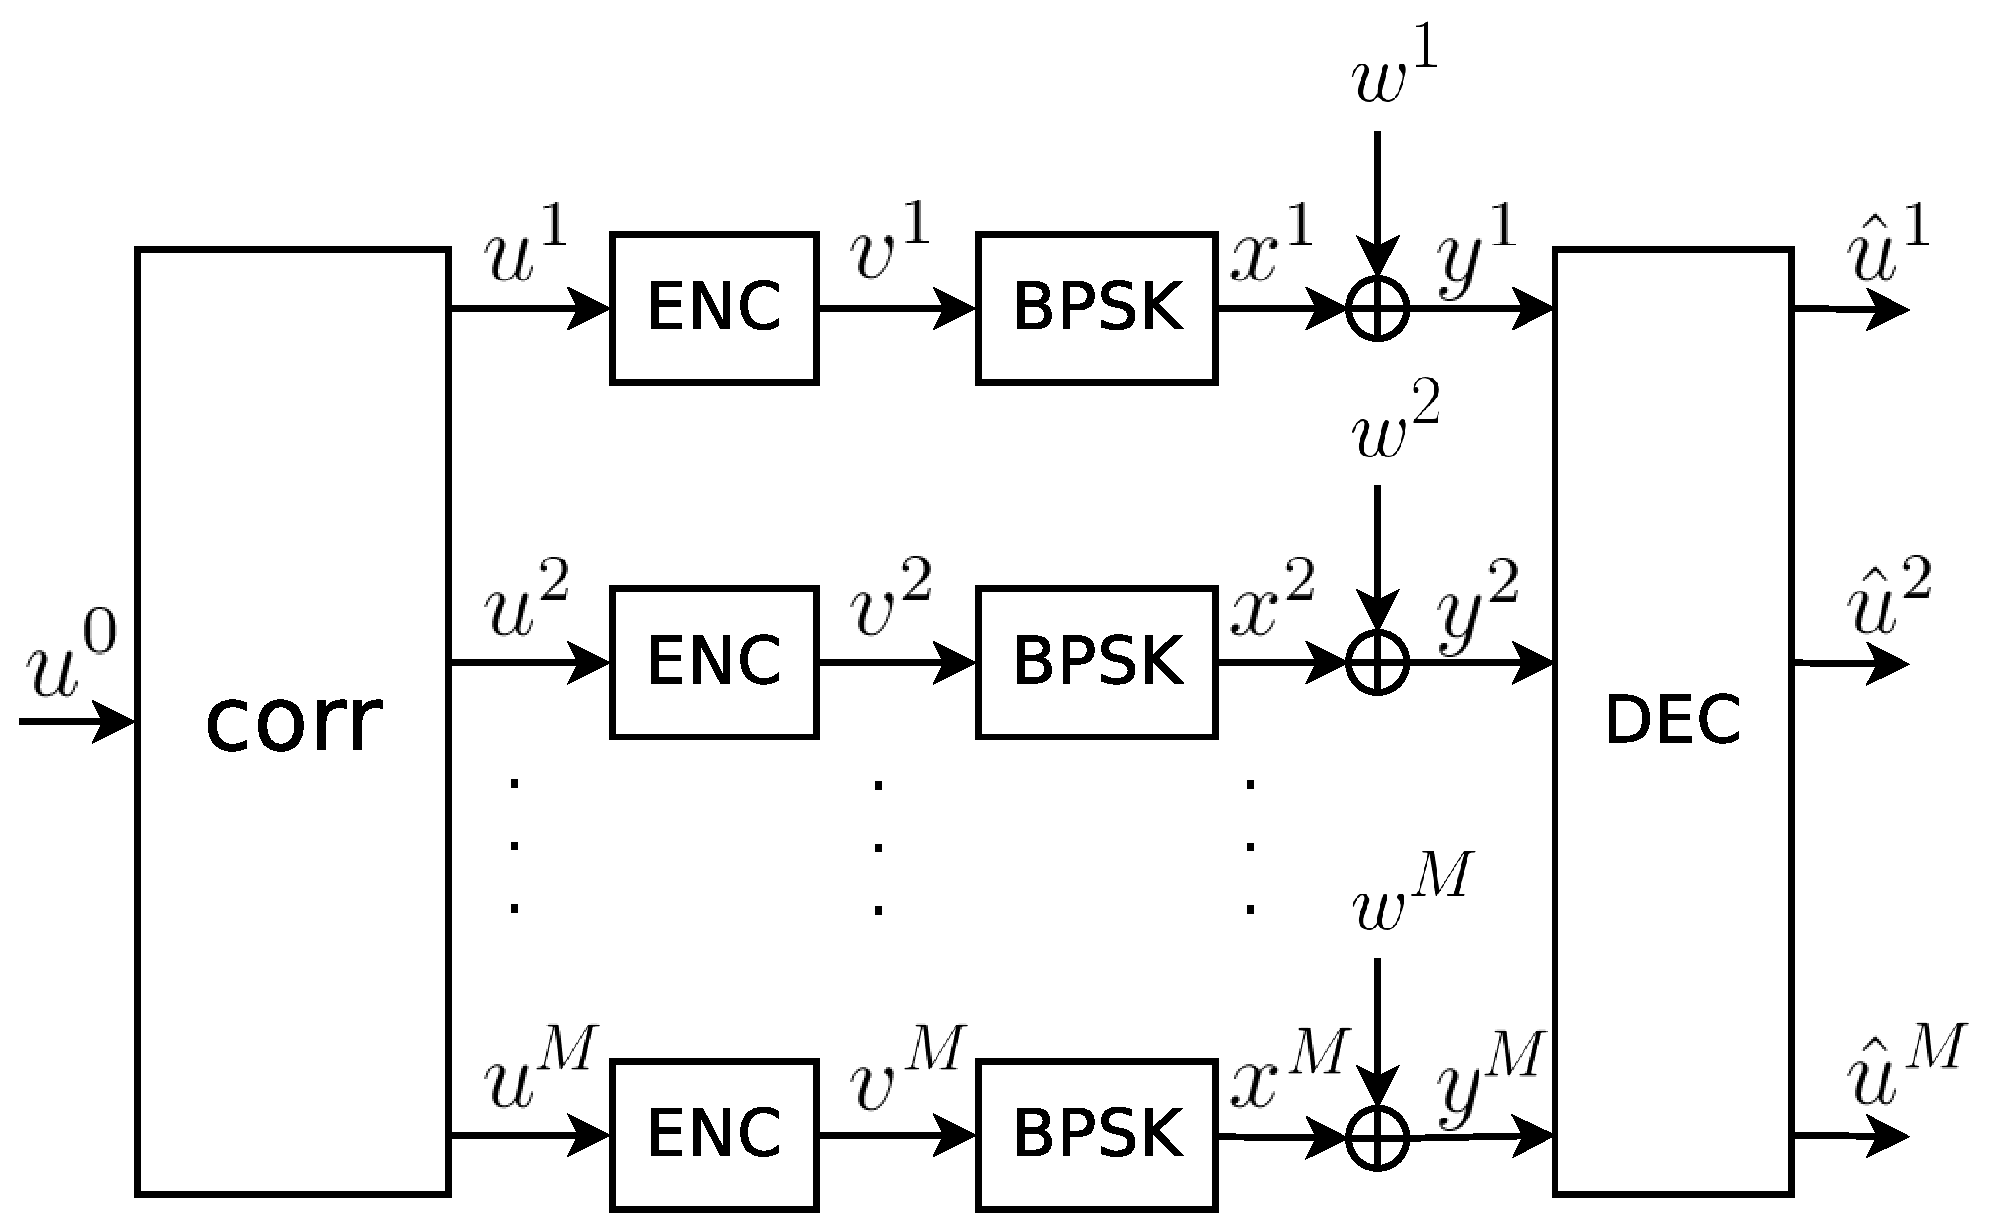
\includegraphics[width=8.6cm]{fig1.eps}
\caption{System Model.} \label{fig:modelo}
\end{figure}

%%Mn the following we drop the upper indexes ``i'' for simplicity. 
Each source vector $\mathbf{u}^{m}$ is encoded into $\mathbf{v}^{m}$,  using a systematic  
Low Density Generator Matrix ($LDGM$) code \cite{art-garciafrias}, $G=[I~P]$, 
where $P$ is a $K\times(N-K)$ sparse matrix (and, therefore, the code rate is $r=K/N$ ).
A codeword at the output of each encoder is mapped with a binary phase shift keying (BPSK) into a 
signaling vector $\mathbf{x}^{m}=(x^{m}_1, \cdots, x^{m}_n, \cdots, x^{m}_{N}) $, 
where $x^{m}_n \in \{\pm 1 \}$, $\forall n\in \{1, 2, \ldots, N\}$, 
and is transmitted on an additive white
Gaussian noise (AWGN) channel. At the receiver, the input to the decoder is
given by $\mathbf{y}^{m}=(y_1^{m}, \cdots, y^{m}_n, \cdots, y^{m}_{N})$, where
$y^{m}_{n}=x^{m}_{n} + w^{m}_{n}$  being $w^{m}_{n}$ an additive white Gaussian
noise with zero mean and variance $\sigma^{2}_{m}=(2E_{s}/N_{0 m})^{-1}$,
 $E_s$ is the energy per transmit symbol and $N_{0m}$  the one-sided
noise spectral density for a $m$-th source. After applying hard-decision on
$\mathbf{y}^{m}$, a vector $\mathbf{z}^{m}=(z^{m}_1, \cdots, z^{m}_n, \cdots, z^{m}_N)$
is obtained. The decoding of  this vector is made using the parity check 
matrix $H=[P^T~I]$, where the super index $T$ indicates the transpose of the matrix $P$.
After error correction decoding over $\mathbf{z}^{m}$, the $K$ first bits of $\mathbf{z}^{m}$ represent an
approximation $\mathbf{\hat{u}}^{m}$ of $\mathbf{u}^{m}$.

%%%%	\subsection{Slepian-Wolf Theorem}
%%%%	\label{Subsubsec:SlepianWolfm}
%%%%	The $Slepian$-$Wolf$ theorem described in \cite{slepian,cover}, show the equation restrictions 
%%%%	for that ${M}$ correlated sources $u^m$, $\forall m \in \{1, ..., M\}$, can send data with an 
%%%%	information rate $\mathrm{R}_m$ so that the information of all sources can be recoverable without error  by common receptor. 
%%%%	For to know these equation restrictions is necessary define first $S \subseteq \{1, 2, ..., {M}\}$ 
%%%%	, $S^c$ as your complement,
%%%%	\begin{equation}\label{eq:RS}
%%%%	R(S) \equiv \sum_{m \in S}{\mathrm{R}_m},
%%%%	\end{equation}and $h(.)$ is the binary entropy function defined in (\ref{eq:hbinary})
%%%%	and
%%%%	\begin{equation}\label{eq:US}
%%%%	U(S) \equiv \bigcup_{m \in S}{u^m}.
%%%%	\end{equation}
%%%%	The $Slepian-Wolf$ theorem show that $\forall S \subseteq \{1, 2, ..., {M}\}$ is valid that
%%%%	\begin{equation}\label{eq:SWmFontes}
%%%%	R(S) \geq H(U(S)|U(S^c)).
%%%%	\end{equation}

%%%%	\begin{comment} [Comment 1]
%%%%	Considering that each subset $S$ have $\tau$ elements, the number of equations per subset is $\binom{{M}}{\tau}$.
%%%%	Them the $Slepian-Wolf$ theorem have in total $\tau_{eq}$ restriction equations, where
%%%%	\begin{equation}\label{eq:Teq}
%%%%	\tau_{eq}=\sum^{{M}}_{t=1}\binom{{M}}{t}=2^{M}-1.
%%%%	\end{equation}
%%%%	For example, in the case that ${M}=100$ the $Slepian-Wolf$ theorem have 
%%%%	$1.26765~10^{30}$ restriction equations.
%%%%	\end{comment}



%%%%%%%%%%%%%%%%%%%%%%%%%%%%%%%%%%%%%%%%%%%%%%%%%%%%%%%%%%%%%%%%%%%%%%%%%%%%%%%%%%%%%%%
%%%%%%%%%%%%%%%%%%%%%%%%%%%%%%%%%%%%%%%%%%%%%%%%%%%%%%%%%%%%%%%%%%%%%%%%%%%%%%%%%%%%%%%
%%%%%%%%%%%%%%%%%%%%%%%%%%%%%%%%%%%%%%%%%%%%%%%%%%%%%%%%%%%%%%%%%%%%%%%%%%%%%%%%%%%%%%%
\section{Bit-Flipping Decoding} \label{sec:BF}

In this section we describe bit-flipping algorithm \cite{kou,galaguer}, 
for obtaining estimations $\mathbf{\hat{u}}^{m}=(\hat{u}_1^{m}, \cdots,$ 
$\hat{u}_k^{m}, \cdots, \hat{u}_{K}^{m}) $, $\forall m \in \{1, 2, \ldots, M\}$, of the 
information transmitted by all sources $u^{m}$ in Fig. \ref{fig:modelo}. In the
algorithm all decoders work in parallel and none 
of the decoders receive side information from others. This algorithm 
will be referred as \textit{independent decoding.}


\subsection{Independent Decoding}
\label{Subsec:AlgDecInd}
In the following we drop the upper indexes ``m'' for simplicity.
Let $H=[h_{l,n}]$ be the parity-check matrix of a $LDGM$ code.
The $l$-th syndrome component is given by the check $s_{l}=\sum_{n} h_{l,n} z_{n}$ (mod 2), 
$\forall l \in \{1, 2, \ldots, (N-K)\}$.
  Denote the set of bits that participates in
each check bit $l$ and the set of checks in which bit $n$ participates by $\mathcal{N}(l)= \{n | h_{l,n}=1\}$ and
$\mathcal{M}(n)= \{ l | h_{l,n}=1\}$, respectively.

In Bit-Flipping ($BF$) decoding \cite{kou,galaguer}, the decoder computes flipping function values
\begin{equation}
i_{n}=\sum_{l\in \mathcal{M}(n)} s_{l},\label{Eq:En1}
\end{equation}
 and flips all bits $z_{n}$ for
which $i_{n} \geq \delta $. New syndromes are re-computed and the
process is repeated until all syndromes equal zero, as in \cite{kou}.
Sipser and Spielman proposed hard-decision algorithms based on a simple criterion:
a bit is flipped if it has  more non-null syndrome values than null ones \cite{sipser}. 
They also show that allowing a limited
amount of negative progress is improved the sequential algorithm. 

In this paper we use a modified version of Sipser and Spielman algorithm allowing any amount of negative
progress. The flipping function is then given by
\begin{equation}\label{Eq:En2}
i_{n}=\sum_{l\in \mathcal{M}(n)} (2 s_{l} - 1)
\end{equation}
for to get the reliability vector $\mathbf{i}=({i}_1, ..., {i}_n, ..., {i}_N)$.
We describe now the modified version: the
Parallel Hard Bit-Flipping (PHBF) Decoding Algorithm \cite{tese}.\\

\begin{algorithm}[PHBF Algorithm]

\begin{enumerate}
\item Initialize $b=0$ and $\mathbf{z}^{(b)}$ $=(z^{(b)}_1, \cdots,$ $z^{(b)}_n, \cdots,$ $z^{(b)}_N)=$ $\mathbf{z}$.

\item Compute the syndrome values $s_{l}=\sum_{n} h_{l,n} z^{(b)}_{n}$ (mod 2), $\forall l \in \{1,\cdots, (N-K)\}$.
If all values are zero then stop decoding since $\mathbf{z}^{(b)}$
is the output codeword.

\item  For $n=\{1,\cdots, N\}$ compute the flipping function $i_{n}$ in (\ref{Eq:En2}).

\item Identify the set of bits $\{ n^{*} \}$
for which $n^{*}=\arg \max_{n} i_{n}$.

\item  Flip  all bits in $\{n^{*} \}$ in parallel. The flipped hard-decision vector is stored in
$\mathbf{z}^{(b+1)}$.

\item If a maximum number of iterations is not reached, set $b \leftarrow b+1$ and go to Step 2).
 Otherwise stop and $\mathbf{z}=\mathbf{z}^{(b+1)}$ is the output codeword.
\end{enumerate}
\end{algorithm}
The Fig. \ref{fig:flowphbf} show a simplify form the last algorithm.
\begin{figure}[!bt]
\centering
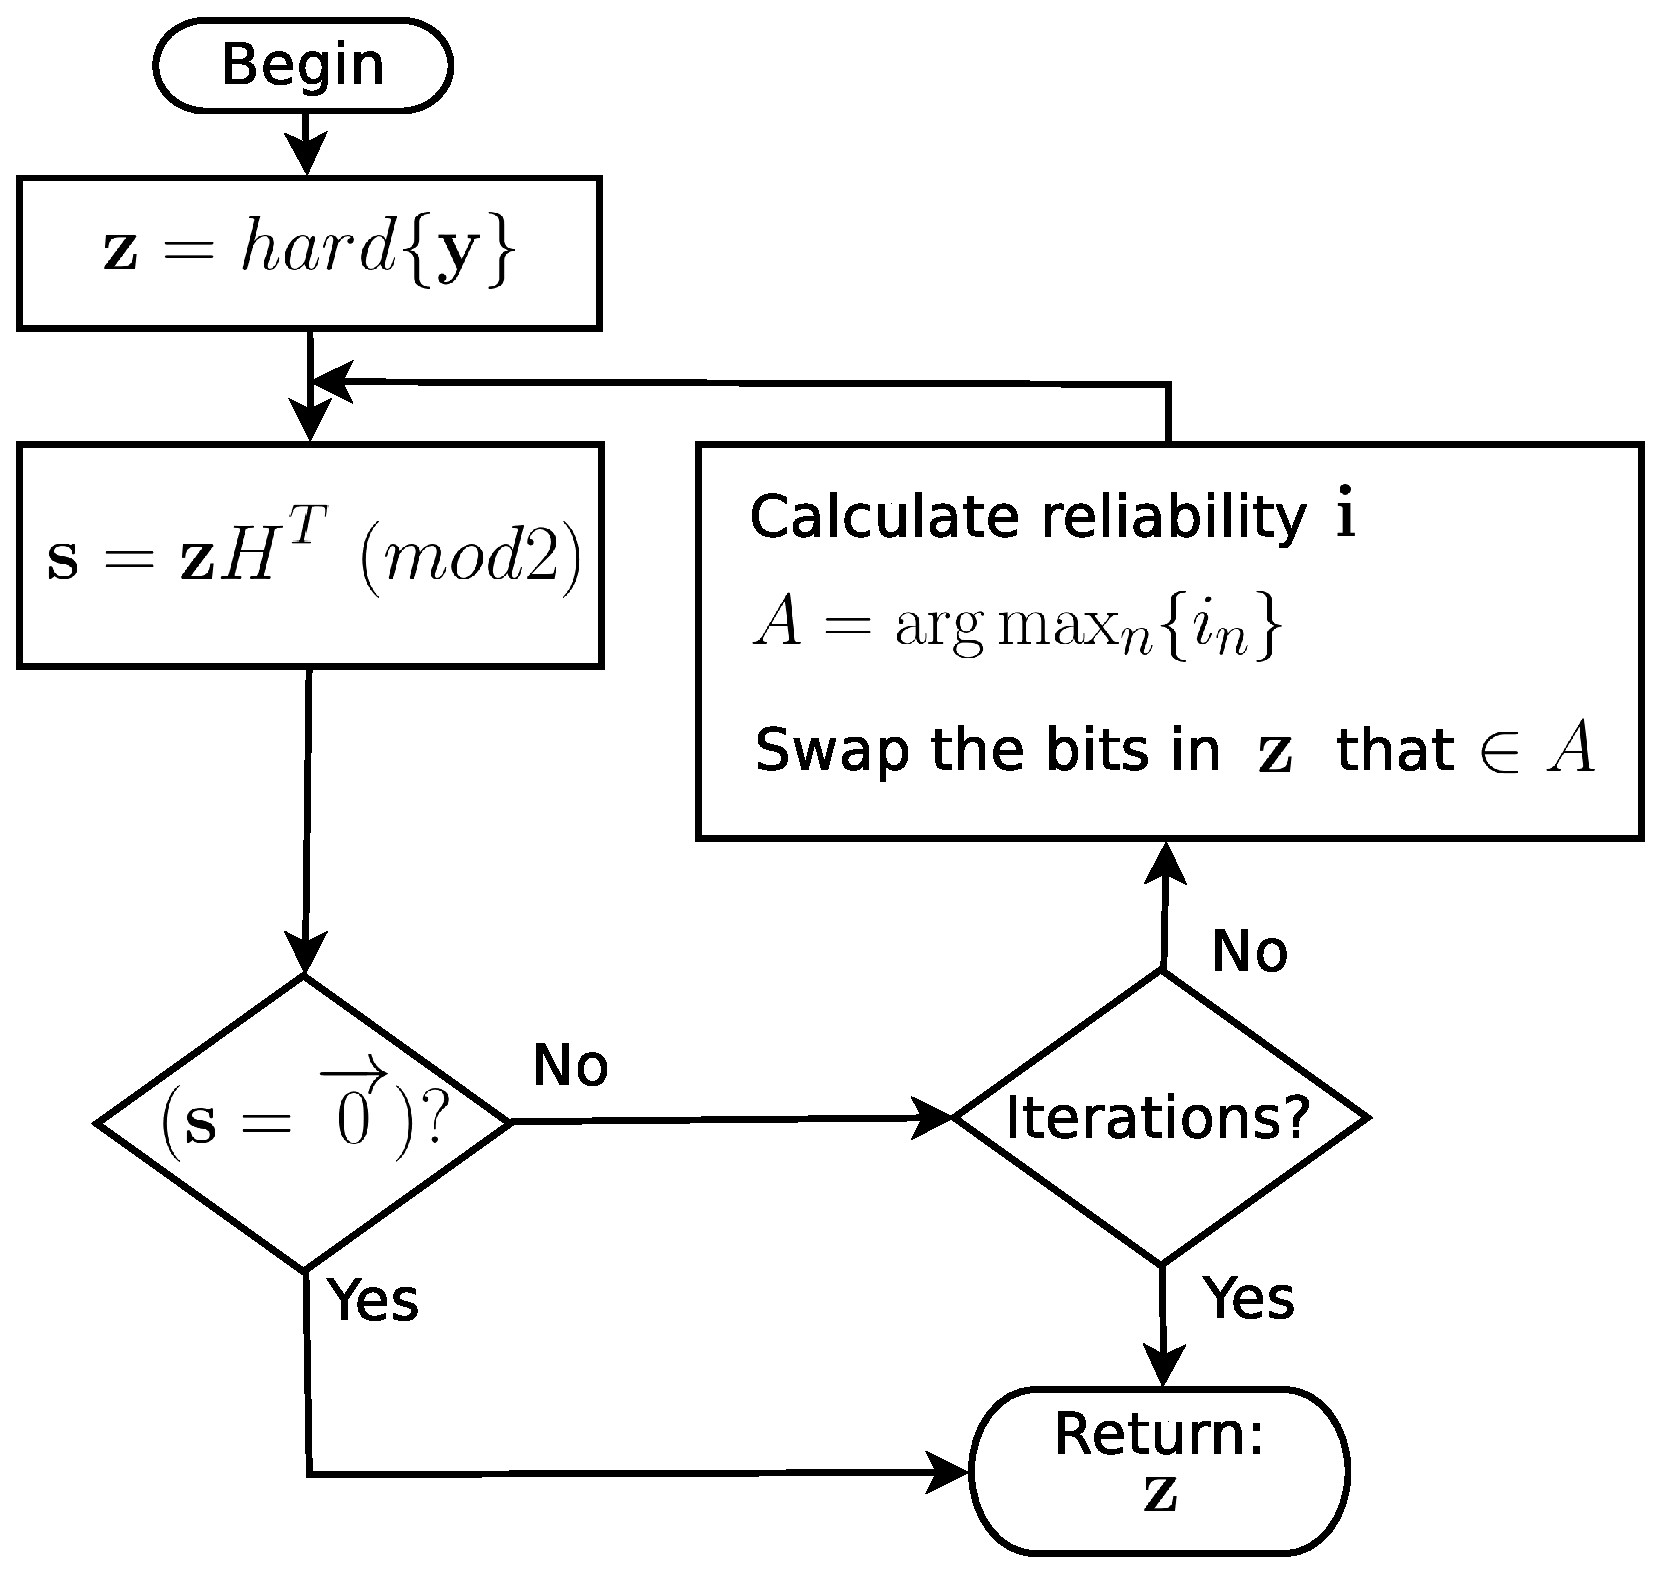
\includegraphics[width=8.6cm]{fig21.eps}
\caption{Flow diagram of Parallel Hard Bit-Flipping algorithm.} \label{fig:flowphbf}
\end{figure}


%%%%%%%%%%%%%%%%%%%%%%%%%%%%%%%%%%%%%%%%%%%%%%%%%%%%%%%%%%%%%%%%%%%%%%%%%%%%%%%%%%%%%%%
%%%%%%%%%%%%%%%%%%%%%%%%%%%%%%%%%%%%%%%%%%%%%%%%%%%%%%%%%%%%%%%%%%%%%%%%%%%%%%%%%%%%%%%
%%%%%%%%%%%%%%%%%%%%%%%%%%%%%%%%%%%%%%%%%%%%%%%%%%%%%%%%%%%%%%%%%%%%%%%%%%%%%%%%%%%%%%%
\section{Distributed Bit-Flipping Decoding} \label{sec:DBFD}

Of similar way of Section \ref{sec:BF}, in this section will be presented an algorithm for
obtaining estimations $\mathbf{\hat{u}}^{m}$, of the 
information transmitted by all sources $u^{m}$ in Fig. \ref{fig:modelo}.  with the difference
that in this algorithm all decoders receive side information from 
others. This algorithm will be called \textit{joint decoding}.

\subsection{Understanding the Joint Decoding}
\label{Subsec:Understanding}

For understanding the joint decoding algorithm, we first should remember that in the 
Section \ref{sec:BF}, the validation of each receive vector $\mathbf{z}^{m}=( z_{1}^{m}$ 
$, \dots, z_{n}^{m} , \dots,z_{N}^{m})$ is analyzed using the flipping function 
$\mathbf{i}^m=({i}^{m}_1, ..., {i}^{m}_n, ..., {i}^{m}_N)$. Thus, in the $m$-th 
source, each couple $\{z_{n}^{m},i_{n}^{m}\}$ represent a reliability ${i}^{m}_n$ 
of that $n$-th bit in $\mathbf{z}^{m}$ be equal to ${z}^{m}_n$. In independent 
decoding for to decide over $\mathbf{z}^{m}$ a horizontal analysis is employed 
for to calculate each element ${i}^{m}_n$ in $\mathbf{i}^m$ $\forall n$ 
$\in \{1, 2, \ldots, N\}$. In the joint decoding a second vertical analysis 
is defined for to obtain the joint reliability vector $\mathbf{j}^m=({j}^{m}_1, ...,$ 
${j}^{m}_n, ..., {j}^{m}_N)$, this second analysis use vertically the couples 
$\{z_{n}^{m},i_{n}^{m}\}$ $\forall$ $m$ $\in \{1, 2, \ldots, M\}$ for to get  
each ${j}^{m}_n$ in $\mathbf{j}^m$, this is side information. 
Thus, in terms of human behavior the independent reliability $\mathbf{i}^m$ 
represent the reliance that one person have in your own solution $\mathbf{z}^m$, and the 
joint reliability $\mathbf{j}^m$ represent the reliance that the others have over 
my solution. Here, we can say that each people use a weighting factor $\beta$
different for to estimate the total reliability 
$\mathbf{t}^m= \mathbf{i}^m + \beta \mathbf{j}^m $, this reliability will be 
the new flipping function. A person that only listening to itself will use only $\mathbf{i}^m$ for to estimate $\mathbf{t}^m$, a person that
don't have reliance in itself will use only $\mathbf{j}^m$ for to estimate $\mathbf{t}^m$.

The calculus of couple $\{z_{n}^{m},j_{n}^{m}\}$ of $n$-th bit in $\mathbf{z}^{m}$,
is similar to case of one student, of a classroom of $M$ students, that go out of test
with one question of true or false type, and find to get the joint reliability  $j_{n}^{m}$,
for your answer $z_{n}^{m}$, knowing the answers and independent reliabilities of the others students. 
Thus, this student decide that the joint reliability  $j_{n}^{m}$ is a weighted average
of independents reliabilities, of the others students, with the reliability that he have
in the answer of other students. In this sense the reliability in the answer of other students 
will be proportional to correlation between these students. Here is necessary to note that for 
calculating the joint reliability  $j_{n}^{m}$, is necessary first homologate the independents
reliability  the others students. This homologation is motivated by the case in that,
in the $a$-th student, the couple $\{z_{n}^{a},i_{n}^{a}\}=\{1,+A\}$  and  in the $m$-th student 
the couple $\{z_{n}^{m},i_{n}^{m}\}=\{0,+B\}$. Thus, the couple of $a$-th student should 
be homologate to $\{z_{n}^{a},i_{n}^{a}\}=\{0,-A\}$, for that both independent reliabilities
talk about your decision of that your bit in study be equal to  zero. In general the homologation rule 
will be that a swap in bit value $z_{n}^{a}$ will be link to sing change in $i_{n}^{a}$.

\subsection{Joint Decoding}
\label{Subsec:AlgDecConj}

The joint decoding algorithm is obtained by modifying the flipping function of the 
independent algorithm.
The new flipping function, $\mathbf{t}^m=({t}^{m}_1, ..., {t}^{m}_n, ..., {t}^{m}_N)$, 
will be the function  
$\mathbf{i}^m=({i}^{m}_1, ..., {i}^{m}_n, ..., {i}^{m}_N)$ given in 
(\ref{Eq:En2}) combined with a joint flipping function, $\mathbf{j}^m=({j}^{m}_1, ..., {j}^{m}_n, ..., {j}^{m}_N)$.
The joint function depends on the bits received by other decoders and also on 
correlations between sources. The new flipping function $\forall n \in \{1, 2, ..., N\}$, in the $m$-th decoder is 
\begin{equation}\label{eq:DSPHBF381}
{t}^{m}_n={i}^{m}_n+ \lfloor \beta  {j}^{m}_n   \rfloor.
\end{equation}
where $\lfloor \alpha \rfloor$ is the greatest integer less than or equal to $\alpha$ and ${j}^{m}_n$ is given by
\begin{equation}\label{eq:DSPHBF1}
{\lambda}^{~}_{m,a,n}=\left \{
\begin{matrix}
-1 & , se & z^m_n \neq z^a_n \\ 
 0 & , se & m=a \\ 
+1 & , se & z^m_n = z^a_n 
\end{matrix}
\right. ,
\end{equation}
\begin{equation}\label{eq:DSPHBF2}
{j}^m_n=\frac{1}{M-1} \sum^{M}_{a=1}{{\lambda}^{~}_{m,a,n}~{i}^a_n ~ corr(u^m,u^a)} ,
\end{equation}

The parameter $\beta$ in (\ref{eq:DSPHBF381}) is to be optimized. If $\beta = 0 $ 
joint decoding becomes independent decoding.
Note that introducing the rounding operation $\lfloor \alpha \rfloor$ leads to a flipping 
function that operates only with integers.
The new algorithm in the joint decoding can be described as\\ \\
\begin{algorithm}[Joint PHBF Algorithm]
\begin{enumerate}
\item Initialize $b=0$ and $\mathbf{z}^{m(b)}$ $=(z^{m(b)}_1, \cdots,$ $z^{m(b)}_n, \cdots,$ $z^{m(b)}_N)=$ $\mathbf{z}^{m}$.

\item Compute the syndrome values $s^{m}_{l}=\sum_{n} h_{l,n} z^{m(b)}_{n}$ (mod 2), $\forall l \in \{1,\cdots, (N-K)\}$, 
and the  flipping function $\mathbf{i}^{m}$ in (\ref{Eq:En2}).
If all syndrome values are zero then stop decoding and return $\mathbf{z}^{m(b)}$ and $\mathbf{i}^{m}$.


\item  Compute the flipping function $\mathbf{t}^{m}$ in (\ref{eq:DSPHBF381}).

\item Identify the set of bits $\{ n^{*} \}$
for which $n^{*}=\arg \max_{n} t^{m}_{n}$.

\item  Flip  all bits in $\{n^{*} \}$ in parallel. The flipped hard-decision vector is stored in
$\mathbf{z}^{m(b+1)}$.

\item If a maximum number of iterations is not reached, set $b \leftarrow b+1$ and go to Step 2).
 Otherwise stop and return $\mathbf{z}^{m}=\mathbf{z}^{m(b+1)}$ and $\mathbf{i}^{m}$. 
\end{enumerate}
\end{algorithm}
The Fig. \ref{fig:flowdphbf} show a simplify form the last algorithm.
\begin{figure}[h!bt]
\centering
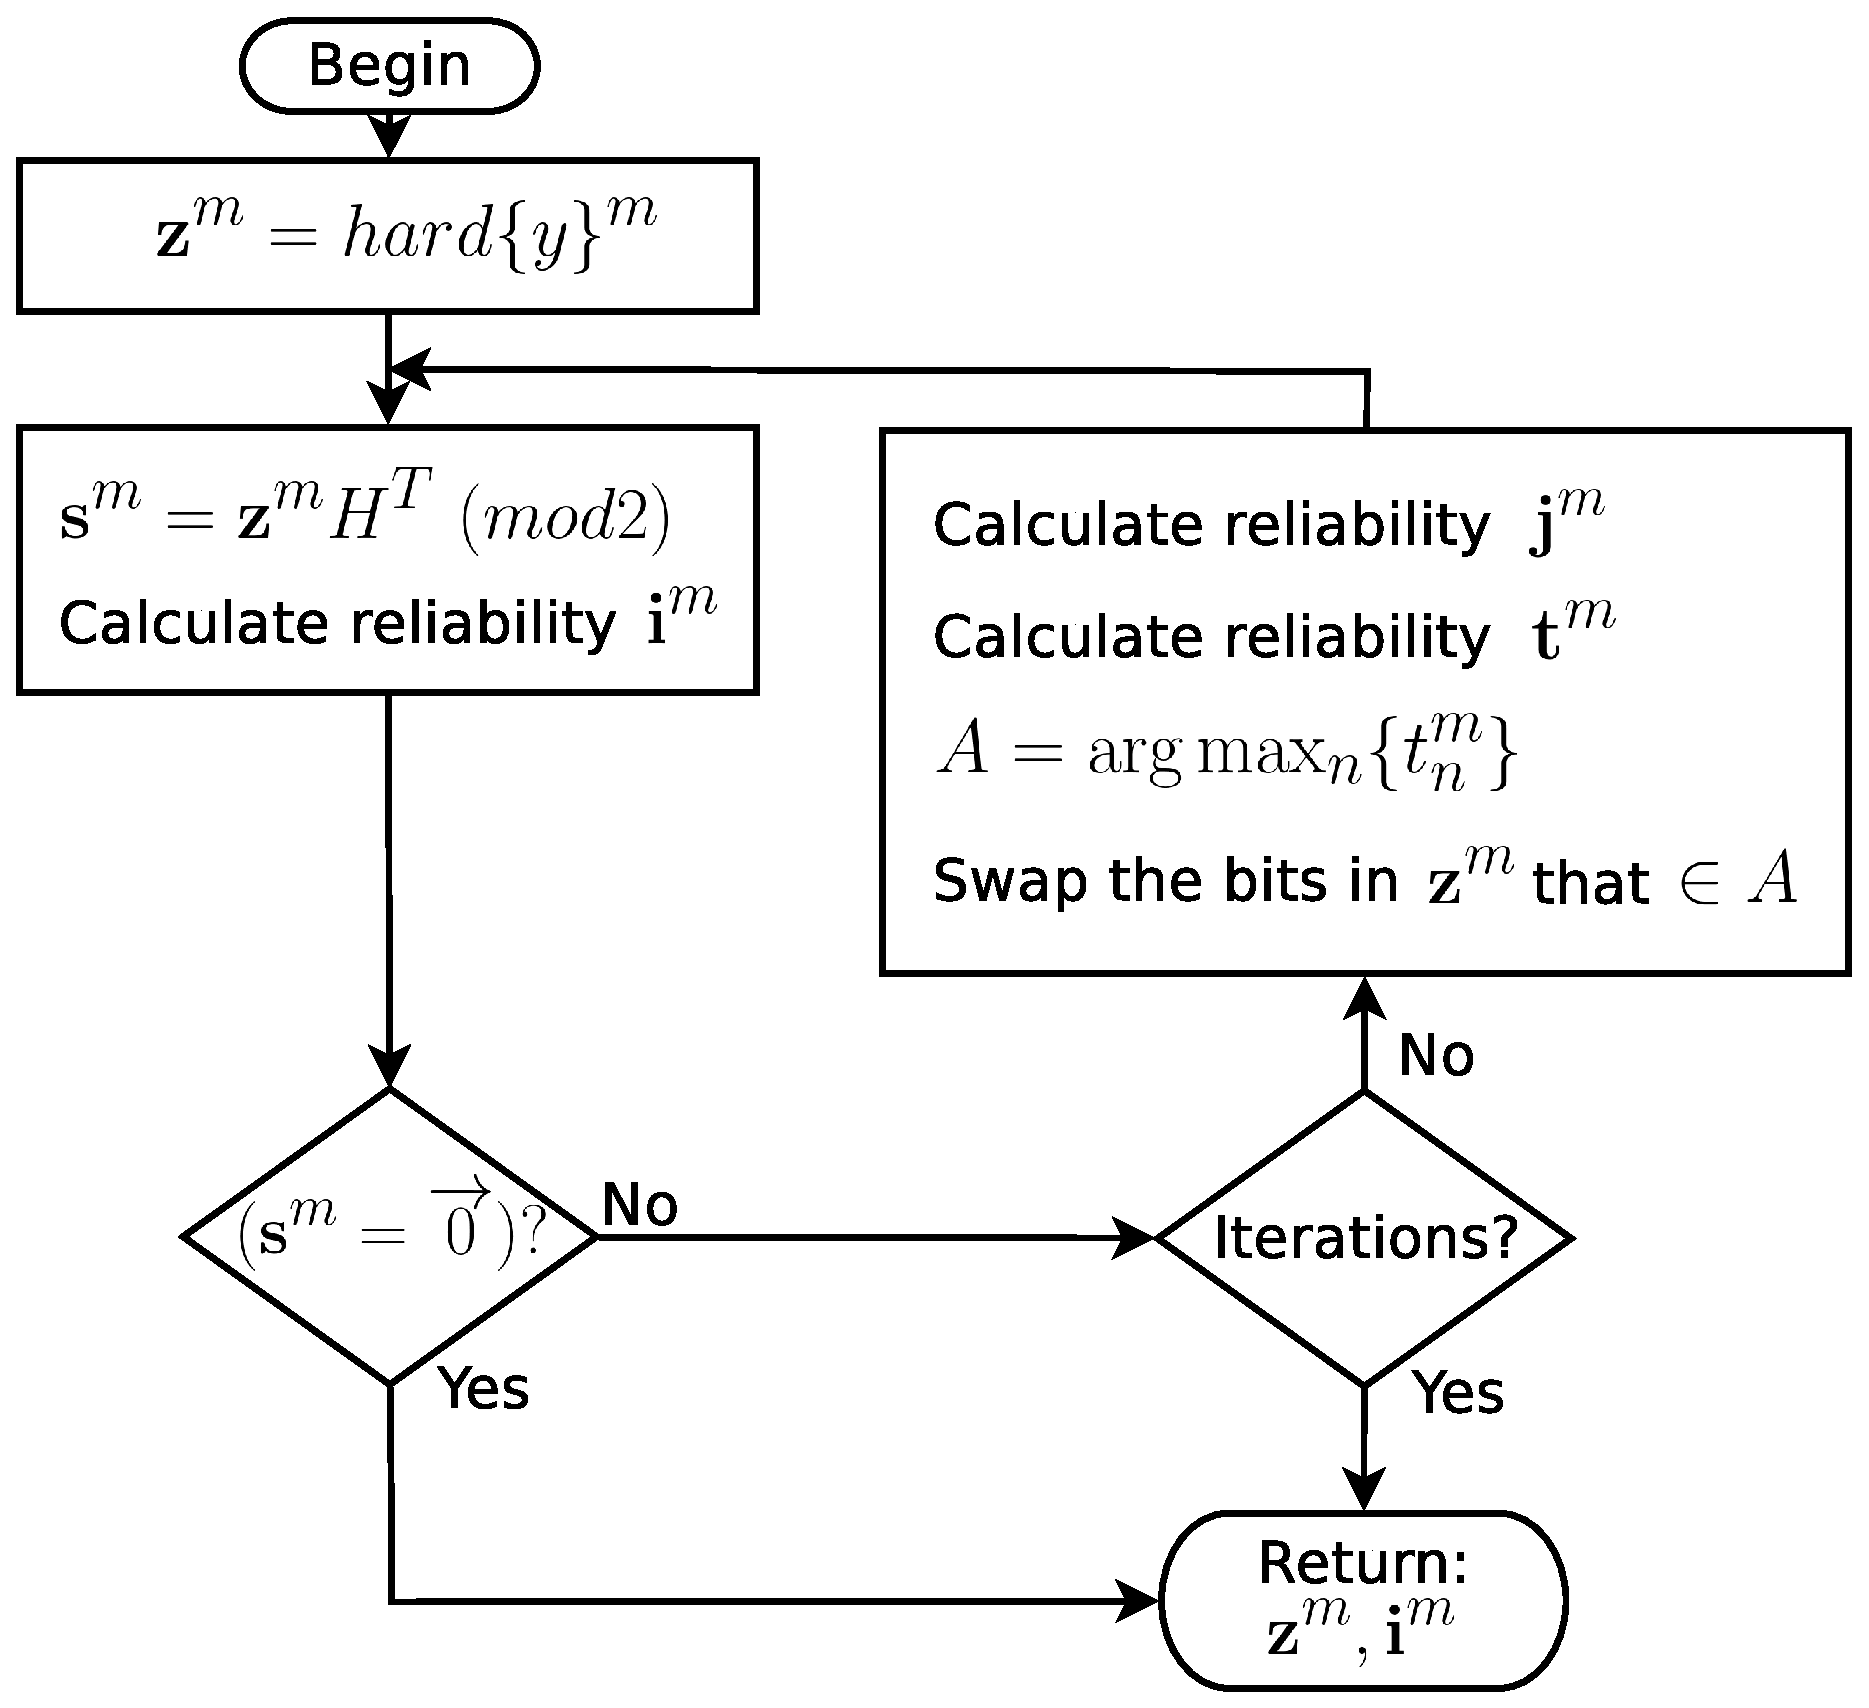
\includegraphics[width=8.6cm]{fig22.eps}
\caption{Flow diagram of distributed Parallel Hard Bit-Flipping algorithm.} \label{fig:flowdphbf}
\end{figure}

\subsection{Joint Decoding Applied to the CEO Problem} 
\label{subsec:ceoproblem}
As is seen in \cite{optimalceo} a good idea for to get a estimation $\hat{u}^0$ 
in the model of the Fig. \ref{fig:modelo},
is to use a criterion of maximum a posteriori (MAP), making the quotient
\begin{equation}\label{eq:ceo_0}
\phi=\frac{P(u^0=1|u^1 u^2 \dots u^{M})}{P(u^0=0|u^1 u^2 \dots u^{M})},
\end{equation}
\begin{equation}\label{eq:ceo_2}
\phi=\frac{P(u^1|u^0=1) P(u^2|u^0=1)  \dots P(u^{M}|u^0=1)}{P(u^1|u^0=0) P(u^2|u^0=0)  \dots P(u^{M}|u^0=0)},
\end{equation}
for to get the $\hat{u}^0$ approximation with
\begin{equation}\label{eq:ceo_1}
\hat{u}^0=
\begin{cases}
1 & \text{ if } \phi > 1 \\ 
0 & \text{ if } \phi \leq 1
\end{cases} ,
\end{equation}

This procedure will be used to obtain the numerical results.
%%%%%%%%%%%%%%%%%%%%%%%%%%%%%%%%%%%%%%%%%%%%%%%%%%%%%%%%%%%%%%%%%%%%%%%%%%%%%%%%%%%%%%%
%%%%%%%%%%%%%%%%%%%%%%%%%%%%%%%%%%%%%%%%%%%%%%%%%%%%%%%%%%%%%%%%%%%%%%%%%%%%%%%%%%%%%%%
%%%%%%%%%%%%%%%%%%%%%%%%%%%%%%%%%%%%%%%%%%%%%%%%%%%%%%%%%%%%%%%%%%%%%%%%%%%%%%%%%%%%%%%
\section{Numerical Results} \label{sec:NumRes}

Numerical results were obtained for scenarios with $M=3$, $M=5$, $M=10$ and $M=100$ sources.
The limit for the bit error rate \cite{art-garciafrias} in independent  decoding  with systematic $LDGM$ matrix is also shown.
In the codewords all the systematic bit nodes have degree $\hat{d}$ and each one of the coded bit nodes has degree 1.

\begin{figure}[h!bt]
\centering 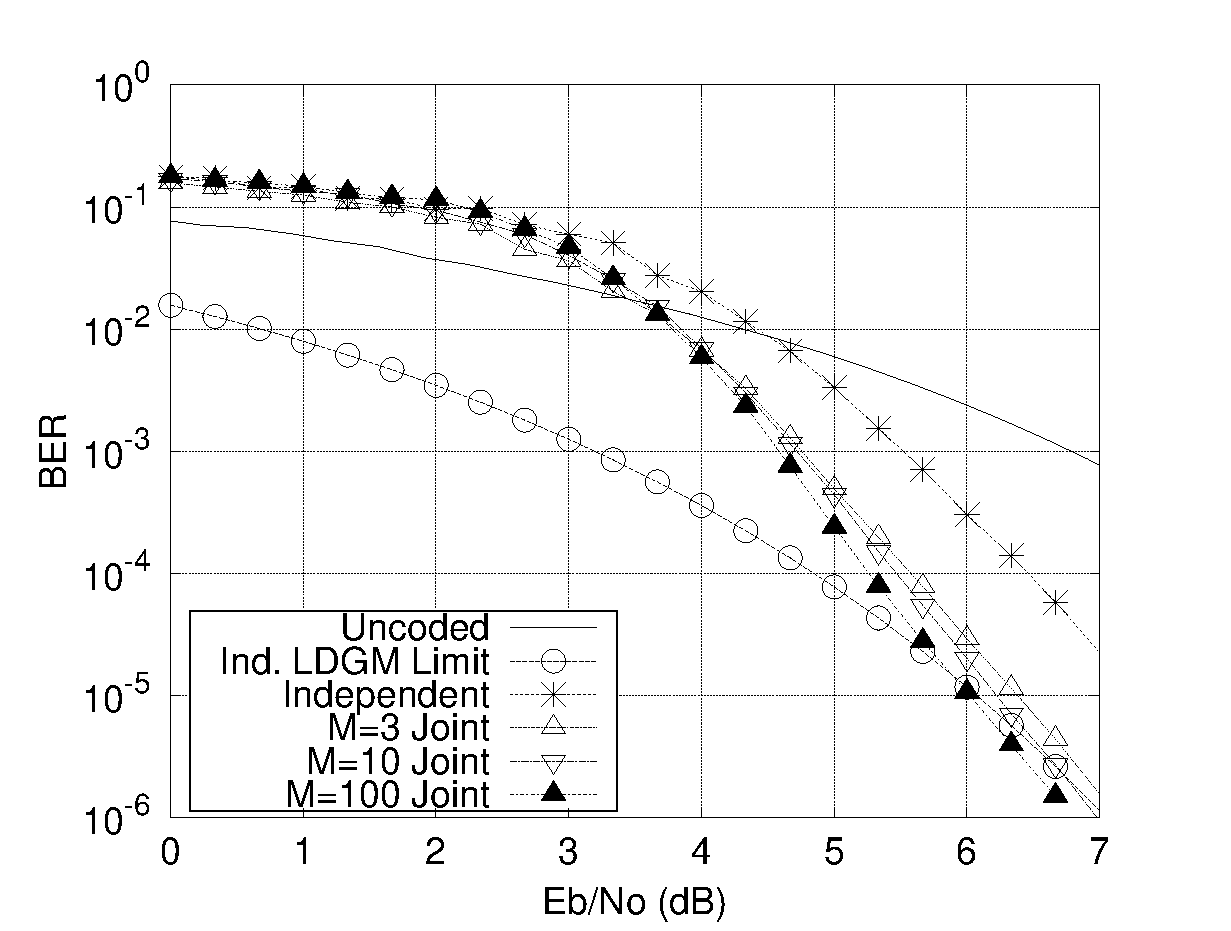
\includegraphics[width=8.5cm]{{./fig2.eps}}
\caption{Bit error rate (BER) for a system with $3$, $10$ and $100$ sources using independent decoding (``Independent'') 
and joint decoding (``Joint''). The limit for the bit error rate  in independent  decoding  with systematic $LDGM$ matrix
(``Ind. LDGM limit'') is also shown.}
\label{fig:fig2}
\end{figure}
Fig. \ref{fig:fig2} compare the average performance of independent and
joint decoding for scenarios with $M=3$, $M=10$ and $M=100$ correlated sources.
A short length systematic $LDGM$ code with parameters $K=204$, $N=306$ and $\hat{d}=5$ were used for encoding the sources.
In the three scenarios, the set of values for the probabilities  $p_{m}=0.1$, $\forall m \in \{1, 2, \ldots, M\}$.
The optimal value obtained for the $\beta$ parameter was $0.6$.
The maximum number of iterations was selected to be equal to $15$. 
As can be seen in the figure, for all scenarios, joint decoding performs better than independent decoding.
The scenario with most number of sources have the better performance, but the improved grows slowly with $M$.


\begin{figure}[h!bt]
\centering 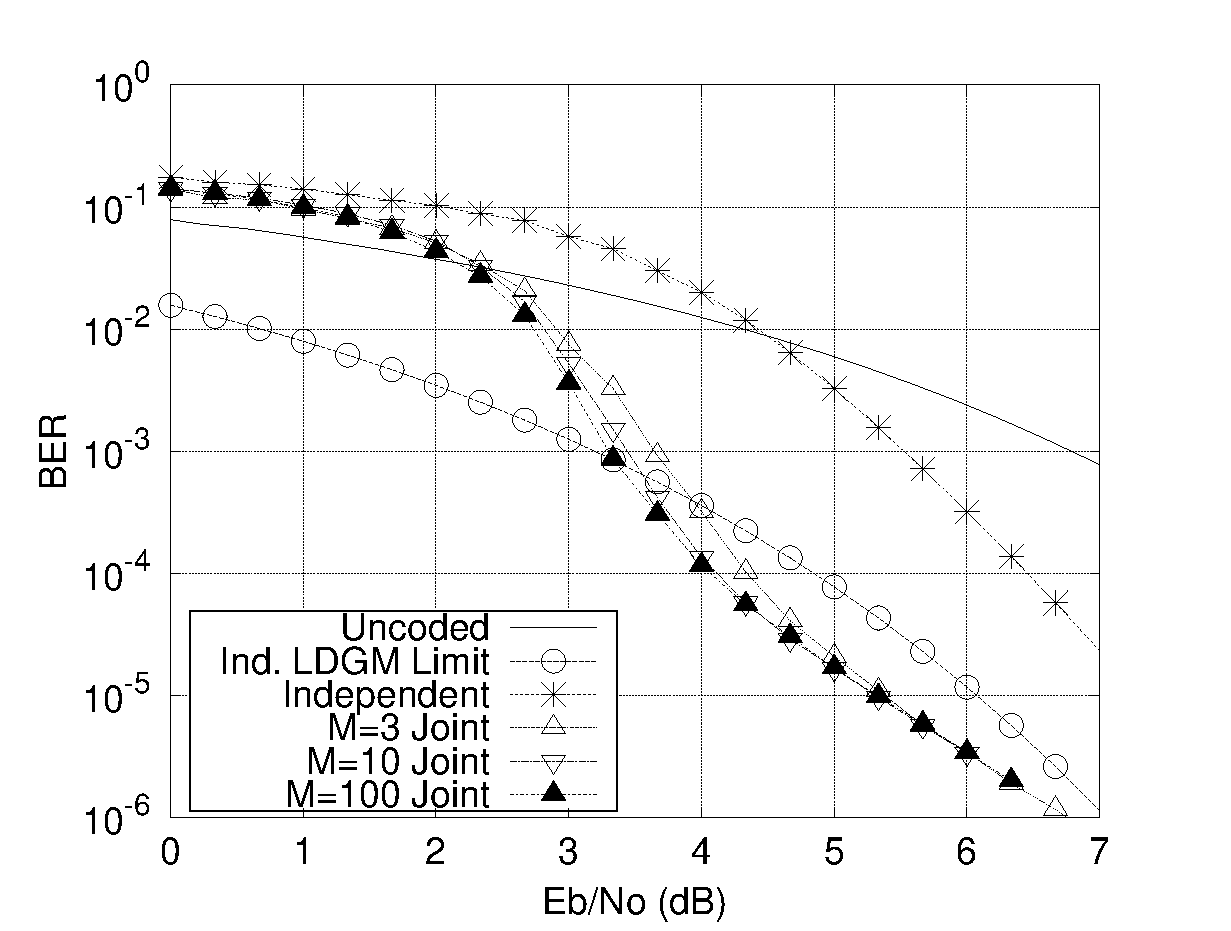
\includegraphics[width=8.5cm]{{./fig2a.eps}}
\caption{Bit error rate (BER) for a system with $3$, $10$ and $100$ sources using independent decoding (``Independent'') 
and joint decoding (``Joint''). The limit for the bit error rate  in independent  decoding  with systematic $LDGM$ matrix
(``Ind. LDGM limit'') is also shown.}
\label{fig:fig2a}
\end{figure}
Fig. \ref{fig:fig2a} compare a case similar to Fig. \ref{fig:fig2} with the same
value of $K$,$N$, $\beta$ parameter and with the 
difference that we have a set of values for the probabilities  $p_{m}=0.005$, 
$\forall m \in \{1, 2, \ldots, M\}$. 


\begin{figure}[h!bt]
\centering 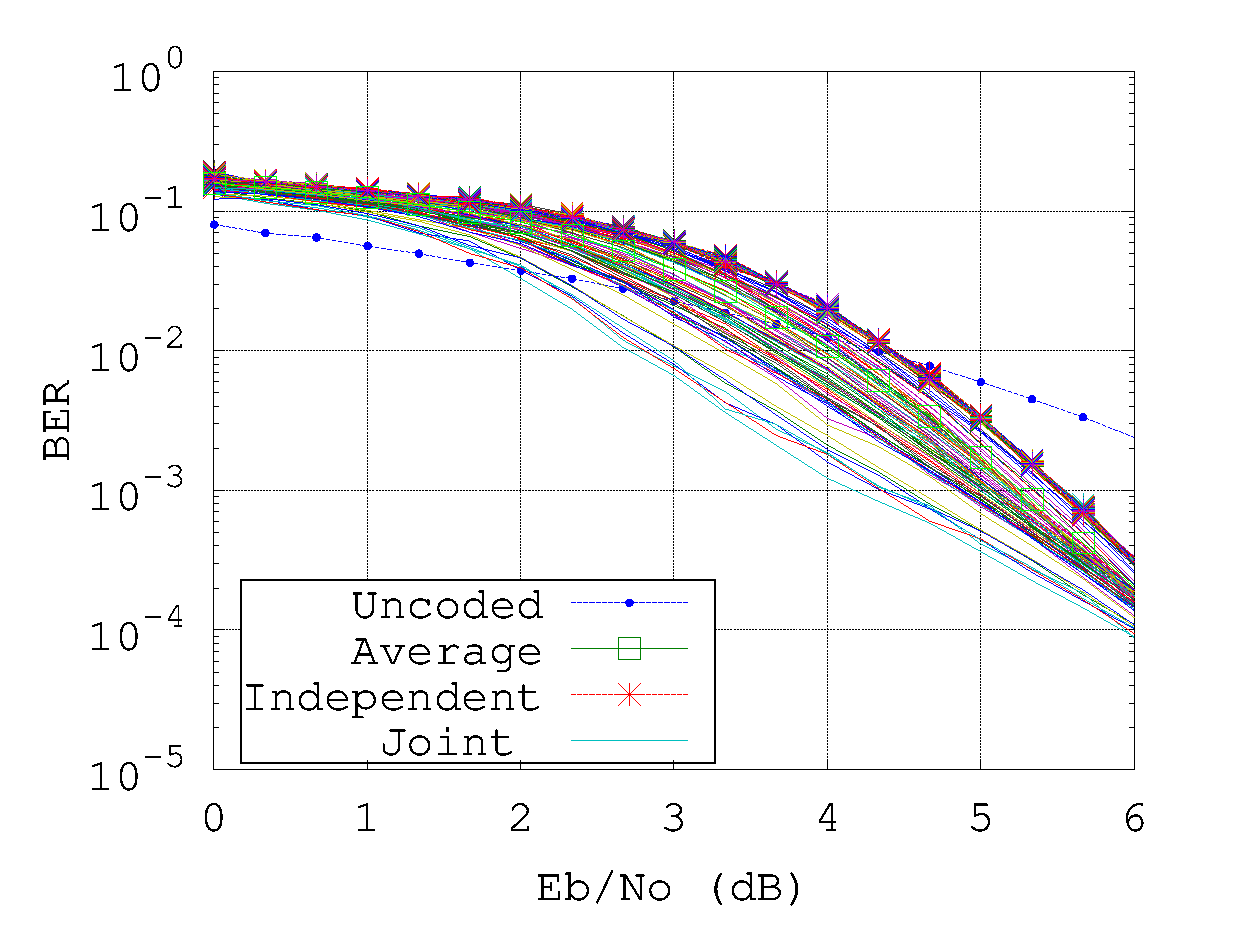
\includegraphics[width=8.5cm]{{./fig3.eps}}
\caption{BER for a system with $3$ sources using independent decoding (``Independent'') and
joint decoding (``Joint''). The limit for the bit error rate  in independent  decoding  with $LDGM$ matrix
(``Ind. LDGM limit'') is also shown.}
\label{fig:fig3}
\end{figure}
Fig. \ref{fig:fig3} compare the performance of independent and
joint decoding for $M=3$ correlated sources.
A long length systematic $LDGM$ code with parameters $K=15000$, $N=30000$ and 
$\hat{d}=9$ were used for encoding the sources.
The set of values for the probabilities are $p_1=p_2=p_3=0.005$.
The maximum number of iterations was selected to be equal to $300$. 
The $\beta$ parameter has been optimized for each value of ${E}_{bm}/{N}_{0m}={E}_{b}/{N}_{0}$.
The Table \ref{tab:1} shows these values. In the Figure can be seen
that joint decoding performs is ever better than independent decoding.
\begin{table}[!hbt]
\caption{Optimal $\beta$ parameter and corresponding ${E}_{b}/{N}_{0}$  in the Fig. \ref{fig:fig3}}
\begin{center}
\begin{tabular}{|l | l | l | l |l | l |}
\hline
${E}_{b}/{N}_{0}$ & $\beta$ & ${E}_{b}/{N}_{0}$ & $\beta$ & ${E}_{b}/{N}_{0}$ & $\beta$   \\
\hline
\hline
2.0 & 0.7 & 2.333 & 0.7 & 2.666 & 0.6 \\
\hline
3.0 & 0.4 & 3.333 & 0.4 & 3.666 & 0.375 \\
\hline
4.0 & 0.3 & 4.333 & 0.2 & 4.666 & 0.2 \\
\hline
\end{tabular}
\end{center}
\label{tab:1}
\end{table}

\begin{figure}[h!bt]
\centering 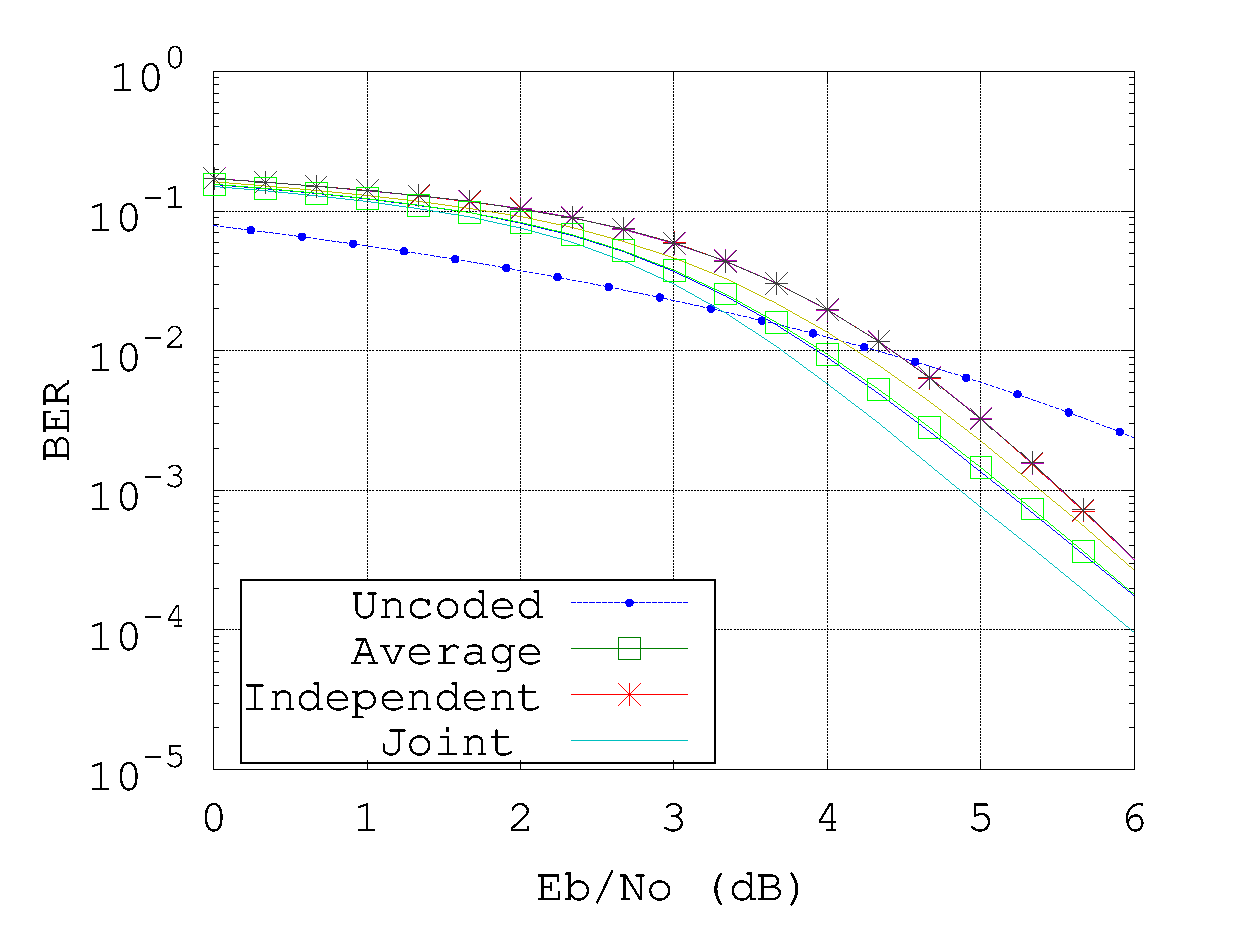
\includegraphics[width=8.5cm]{{./fig4.eps}}
\caption{BER for a system with $5$ sources using independent decoding ("Independent"),
joint decoding ("Joint") and the average bit error rate for joint decoding ("Average").
 The limit for the bit error rate  in independent  decoding  with $LDGM$ matrix
("Ind. LDGM limit") is also shown.}
\label{fig:fig4}
\end{figure}
Fig. \ref{fig:fig4} compare the performance of independent and
joint decoding for $M=5$ correlated sources.
In this figure was used the same systematic $LDGM$ matrix and the maximum number 
of iterations that in the Fig. \ref{fig:fig2}. 
The set of values for the probabilities  $p_{m}$, $\forall m \in \{1, 2, \ldots, 5\}$, are
distributed according the Table \ref{tab:2}, being the minimum value of $p_{m}$
equal to $0.0001$ and the maximum value $0.2$.
The value used in the $\beta$ parameter was $0.6$.
As can be seen in this figure, there are 5 different curves named ``joint'', this happen
because each source $u^m$ have a different error probability $p_{m}$, thus the performance
of each curve is different. In all sources the joint decoding performs are ever better 
than independent decoding. The figure also show a average performance of all joint decoding,
this curve is plotted with $\triangle$.
\begin{table}[!hbt]
\caption{Probability $p_{m}$ and correlation in the distributed source model in the Fig. \ref{fig:fig4}.}
\begin{center}
\begin{tabular}{|l |l | l | l | l |l |}
\hline
~     &$p_1$   & $p_2$  & $p_3$  & $p_4$  & $p_5$   \\
\hline
\hline
$p_{m}$              & 0.0001 & 0.05 & 0.1 & 0.15 & 0.2\\
\hline
$corr(u^{0},u^{m})$& 0.9998 & 0.9  & 0.8 & 0.7  & 0.6\\
\hline
\end{tabular}
\end{center}
\label{tab:2}
\end{table}


\begin{figure}[h!bt]
\centering 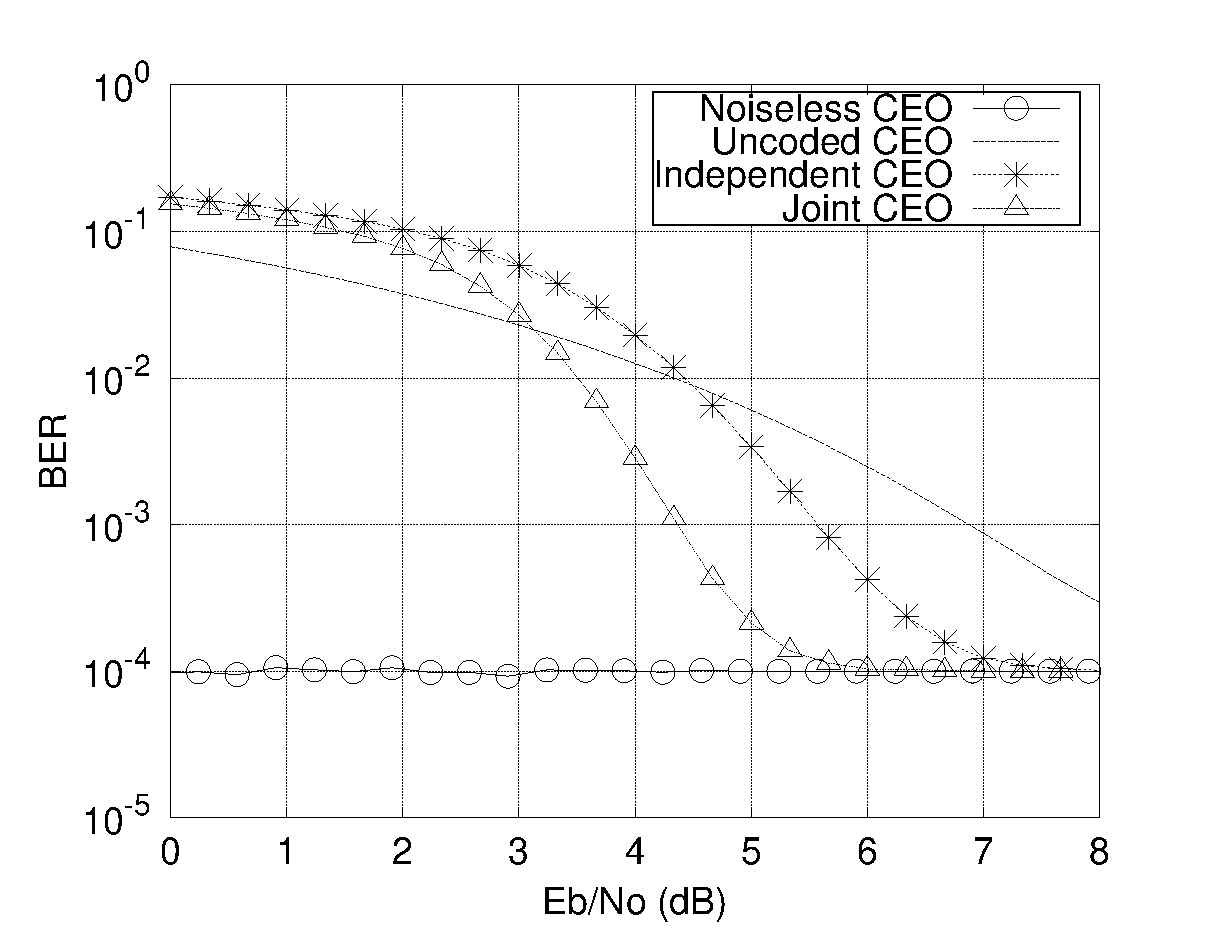
\includegraphics[width=8.5cm]{{./fig5.eps}}
\caption{BER in the estimation $\hat{u}^0$ of $u^0$ for a system with $5$ sources using 
the data after independent decoding (``Independent CEO''),
joint decoding (``Joint CEO''), uncoded data (``Uncoded CEO'') 
and noiseless channel data (``Noiseless CEO'').}
\label{fig:fig5}
\end{figure}
Fig. \ref{fig:fig5} compare the performance in the estimation $\hat{u}^0$ of $u^0$
for the $M=5$ correlated sources seen in Fig. \ref{fig:fig4}.
The algorithm used in the estimation is described in 
the Section \ref{subsec:ceoproblem}. In the figure, can be seen 
the estimation CEO for many cases. Exist the case in 
that the data used for the  CEO estimation is obtained after the joint decoding 
(Joint CEO), also the case when the information is obtained after the independent 
decoding (Independent CEO) or the case in that the information used was obtained 
after  to receive uncoded data (Uncoded CEO). Also we have the ideal case in 
that the data used passes through noiseless channels (Noiseless CEO). The better 
performance is reached for the ``Joint CEO'' estimation, but this
happen only after ${E}_{bm}/{N}_{0m}=3.1dB$. The reason for this is 
that between all sources, the source $u^1$ have better performance
and this source also is  better than uncoded performance  after ${E}_{bm}/{N}_{0m}=3.1dB$.
Known also that the correlation between $u^1$ and $u^0$ 
is very close to one, the source $u^1$ is dominant in the CEO estimation.

\section{Final Remarks and Conclusions} \label{sec:Conclusions}

It was observed in the simulation results that the source $u^{m}$, with highest absolute value 
of the correlation $corr(u^{0},u^{m})$ is recovered with the lowest value of BER
in the joint algorithm. 

By comparing the results in Fig. \ref{fig:fig2a} and Fig. \ref{fig:fig3}
is interesting show that in both graphics the joint decoding curves accompanying
the curve of independent LDGM limit described in \cite{art-garciafrias}. This
is interesting because highlights the possibility of existence of a similar limit 
for the case of distributed sources.

By comparing the results in Fig. \ref{fig:fig4} for the decoder with best 
performance, it can be seen that for $E_{b}/N_{0}$ values  higher than $4$ dB 
leads to significantly better results. 
It is not difficult to show that the source $u^{m}$ of higher  absolute value 
of correlation $corr(u^{0},u^{m})$, is the same that of the greatest  
mutual information $I(u^{0},u^{m})$. However, 
in the system model of Section \ref{sec:SystemModel}, source $u_{0}$ plays the role 
of a common hidden source \cite{raheli2012}.  This implies that in a real situation 
one cannot estimate the mutual information $I(u^{0},u^{m})$.


%%%%% Let $\textbf{u}^{m}_{c}=(u^{1},\ldots,u^{m-1},u^{m+1},\ldots,u^{M})$ be a vector 
%%%%% representing all source variables excluding the $m$-th source. It is reasonable to 
%%%%% argue that the source with the highest value of the joint mutual information 
%%%%% $I(u^{m}, \textbf{u}^{m}_{c})$ should be recovered with the lowest value of BER
%%%%% in the joint algorithm. 
%%%%% Instead of calculating $I(u^{m}, \textbf{u}^{m}_{c})$ we obtained the sum
%%%%% \begin{equation}\label{eq:sum}
%%%%% MI(m)=\sum_{\substack{a=1 \\ a\neq m}}^{M} I(u^{m},u^{a}).
%%%%% \end{equation}
%%%%% In many sets tested of randomly generated correlation values, the highest 
%%%%% value of $MI(m)$ indicated the source recovered with the lowest value of 
%%%%% BER in the joint algorithm.

We have also obtained performance results 
%for all three scenarios described in Section \ref{sec:BF} 
using different sets of values for the probabilities $p_{m}$. It was 
observed that the performance is highly dependent on the choice of these sets 
for the source model.  However, for the scenario of Fig. \ref{fig:fig4}, the lowest value 
of BER was always attained by the sources whose correlation values were intentionally 
selected to be approximately equal to one. These scenarios can be considered as an instance 
of decoding with multiple side information \cite{side}.

If one is interested in estimating the single hidden binary source $u^{0}$, the problem 
considered in this paper becomes an instance of
the binary central estimating officer (CEO) problem \cite{binaryceo}.  Although the 
proposed algorithm do not make any estimation of log-likelihood ratios, 
The data in out of the decoders is used together with the rule 
of the Section \ref{subsec:ceoproblem} for solving this problem.

We have proposed a bit-flipping decoding algorithm suitable for decoding multiple 
correlated sources over noisy channels. The complexity of the proposed  algorithm 
is adequate to be used with a large number of correlated sources.  Performance results 
were obtained for hard-decision bit-flipping decoding algorithms. The proposed 
algorithm can be easily extended for decoding with soft-decisions.

\section*{Acknowledgment}
This work was supported in part by The --------- --------- --------- --------- 
---------  --------- --------- --------- %%%%State of Sao Paulo Research Foundation (FAPESP) under grant 2012/22641-5.

\begin{thebibliography}{1}

%%H(M,\rho)
\bibitem{raheli2011} A. Abrardo, G. Ferrari, and M. Martal\`o,\emph{On non-cooperative 
block-faded orthogonal multiple access schemes with correlated sources}, IEEE Trans. Commun., vol. 59, no. 7, pp. 1916 1926, July 2011.

%%H(M,\rho)
\bibitem{raheli2012}  G. Ferrari, M. Martal\`o, A. Abrardo,  and R. Raheli,
\emph{Orthogonal Multiple Access and Information Fusion: How Many Observations Are Needed?}, 
in Proc. Inform. Theory and Applications Workshop (ITA), UCSD, San Diego, CA, USA, February 2012.

%%Grafo fator, sem codigo, muitas fontes, correlacao gausiana
\bibitem{joao} J. Barros and  M. T$\ddot{u}$chler,\emph{ Scalable Decoding on Factor Trees: A Practical Solution for Wireless Sensor Networks},
IEEE Trans. Commun., vol. 54, no. 2, pp. 284-294, Feb. 2006.


%% slepian wolf e nodos comunicandose
\bibitem{joao1} J. Barros and S. D. Servetto,\emph{Network information flow with correlated sources}, 
IEEE Trans. Inform. Theory, vol. 52, no. 1, pp. 155-170, January 2006.

%%slepian wolf original
\bibitem{slepian}D. Slepian and J. K.Wolf, \emph{A coding theorem for multiple access channels
with correlated sources}, Bell Syst. Tech. J., vol. 52, no. 7, pp.
1037-1076, 1973.

\bibitem{kou} Y. Kou, S. Lin and M. Fossorier, \emph{Low-density parity-check codes
based on finite geometries: a rediscovery and new results}, IEEE
Trans. Inform. Theory, vol. 47, pp. 2711-2736, Nov. 2001.

%% \bibitem{cover}
%% T. M. Cover, and J. Thomas, \textit{Elements of Information Theory}, Wiley-Interscience, 2006.

\bibitem{galaguer} Gallager, R.G., \emph{Low-density parity-check codes}, 
Information Theory, IRE Transactions on , vol.8, no.1, pp.21,28, January 1962


%%CEO , \rho constante, BER(CEO) 
\bibitem{binaryceo} J. Haghighat, H. Behroozi, and D.V. Plant, 
\emph{Iterative joint decoding for sensor networks with binary CEO model}, 
IEEE 9th Workshop on Signal Processing Advances in Wireless Communications, July 2008,
Recife, Brazil.

%% slepian wolf com ruido
\bibitem{japao} K. Kobayashi, T. Yamazato and M. Katayama,\emph{Decoding of Separately Encoded Multiple Correlated Sources Transmitted over Noisy Channels},
  IEICE Trans. Fundamentals,  vol. E92-A ,  no 10,pp 2402-2410, October 2009.

  
  
\bibitem{side}S. Shamai and S. Verdu,\emph{Capacity of channels with uncoded side information}, European Trans. Telecommun., vol. 6,
no. 5, pp. 587-600, September-October 1995.

\bibitem{tese} --------- --------- --------- --------- --------- --------- --------- 
--------- --------- --------- --------- 
%%%%F. Pujaico, Hard decision algorithms for LDGM Codes, (In portuguese),
%%%%Master Thesis, State University of Campinas, Brazil, p. 55, 2011, Available: http://www.bibliotecadigital.unicamp.br.


\bibitem{art-garciafrias} J. F. Garcia-Frias e W. Zhong, \emph{Approaching Shannon performance by
iterative decoding of linear codes with low-density generator matrix,}
~\textit{IEEE Commun. Lett.}, v. 7, n. 6, pp. 266-268, Junho 2003.





\bibitem{sipser} M. Sipser and D. Spielman, \emph{Expander codes}, IEEE Trans. Inform.
Theory, vol. 42, pp. 1710-1722, Nov. 1996.

\bibitem{optimalceo} Chair, Z.; Varshney, P.K., ``Optimal Data Fusion in Multiple Sensor Detection Systems,'' 
Aerospace and Electronic Systems, IEEE Transactions on , vol.AES-22, no.1, pp.98,101, Jan. 1986


\end{thebibliography}

\end{document}
